\section{A concrete implementation of REAR}
\label{sec:concr}

blah blah

\subsection{Data source}

\subsection{Metrics}

\subsubsection{The spacial metric algorithm}
\label{subsec:spacial_metric_algorithm}

\begin{figure}[!h]
  \begin{center}
    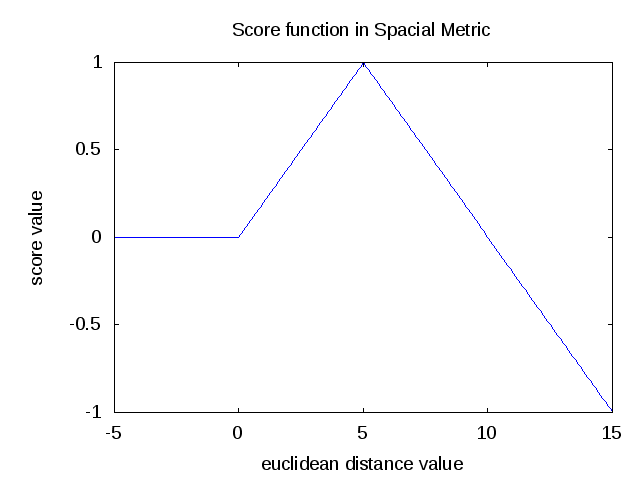
\includegraphics[width=400pt]{img/spacialMetricFunc.png} 
    \caption{Spacial Metric Function}
    \label{fig:spacial_metric_func}
  \end{center}
\end{figure}

This algorithm uses a simple triangle function to couple the image processed with a score.
%

%
The distance value between robot and image is processed by a triangle function. User specifies
the optimal distance between image and robot, that is the distance value where
the score function return the maximum value and therefore where the triangle is centred.
In figure \ref{fig:spacial_metric_func} the optimal distance is set to 5.
%

%
Since the \texttt{DataLogic} object will select the image coupled with the minimum value, we have
to invert the score sign before returning it.
%

%
This algorithm does not care about image orientation. For instance, it could choose an image that
does not include the robot from its point of view. This limit makes the algorithm good only for
quite linear route taken by the robot, but bad for more complex ones. On the other hand, its
implementation is very simple.
%

%
The \texttt{Sweep Metric Algorithm} in chapter \ref{subsec:sweep_metric_algorithm} will try to
go behind this limits.


\subsubsection{The sweep metric algorithm}
\label{subsec:sweep_metric_algorithm}
The "sweep angle" algorithm allows to choose the better background image, in order to implement
the exocentric vision.
%
\begin{figure}[!h]
  \begin{center}
    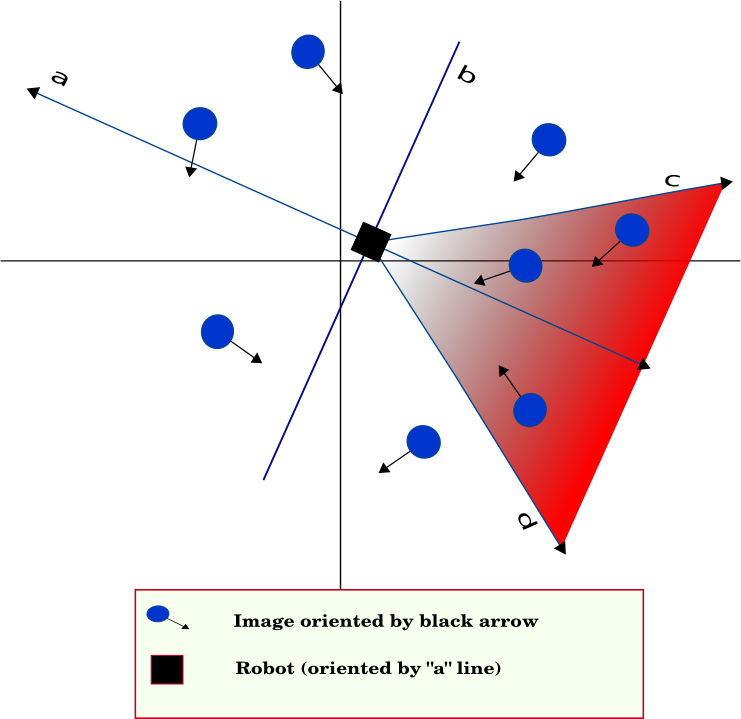
\includegraphics[width=400pt]{img/half_plan_finding.png} 
    \caption{Sweep Angle Algorithm}
    \label{fig:half_plan_finding}
  \end{center}
\end{figure}
%
All the explanation will refer to image \ref{fig:half_plan_finding}. In the latter, the black
square represents the robot, with its orientation indicated by the arrow "a", starting from the
square.
%

%
The several blue circles represent instead the previous shoot images. The orientation of each
image (i.e. the orientation of the robot when they were shoot) is shown by an arrow starting from
each circle.
%

%
We will refer to the line perpendicular to the half line "a" as "b". By rotating clockwise and
counterclockwise the "a" line in the robot centre with a predefined angle (named "sweep angle")
we will obtain the "c" and "d" lines. These define a new portion of the plane (coloured with fading red),
named the "sweep area".
%

%
Since we want to control the robot from the rear position, the sought image will be included within
this area: all the other ones will be discarded. Even tough this method allows us to exclude many
images, the selection is certainly not over.
%

%
First of all, we have to discard all the images with an orientation angle that differs too much from the
robot orientation angle. If the difference between the two angles is greater than a specified threshold,
the image can not be chosen as background, because the latter does not include the robot from its point
of view. For instance, if the difference angle between the robot and the image orientation is 180 degrees,
it means that robot and camera are oriented in opposite way, therefore the camera can not see the robot
itself.
%

%
After excluding the badly oriented images, we proceed with the score assignment. The latter is obtained by
the sum of two factors. The first takes in account the image angle orientation: the more the image orientation
angle is close to the robot orientation angle, the more the score is high.
%
\begin{figure}[!h]
  \begin{center}
    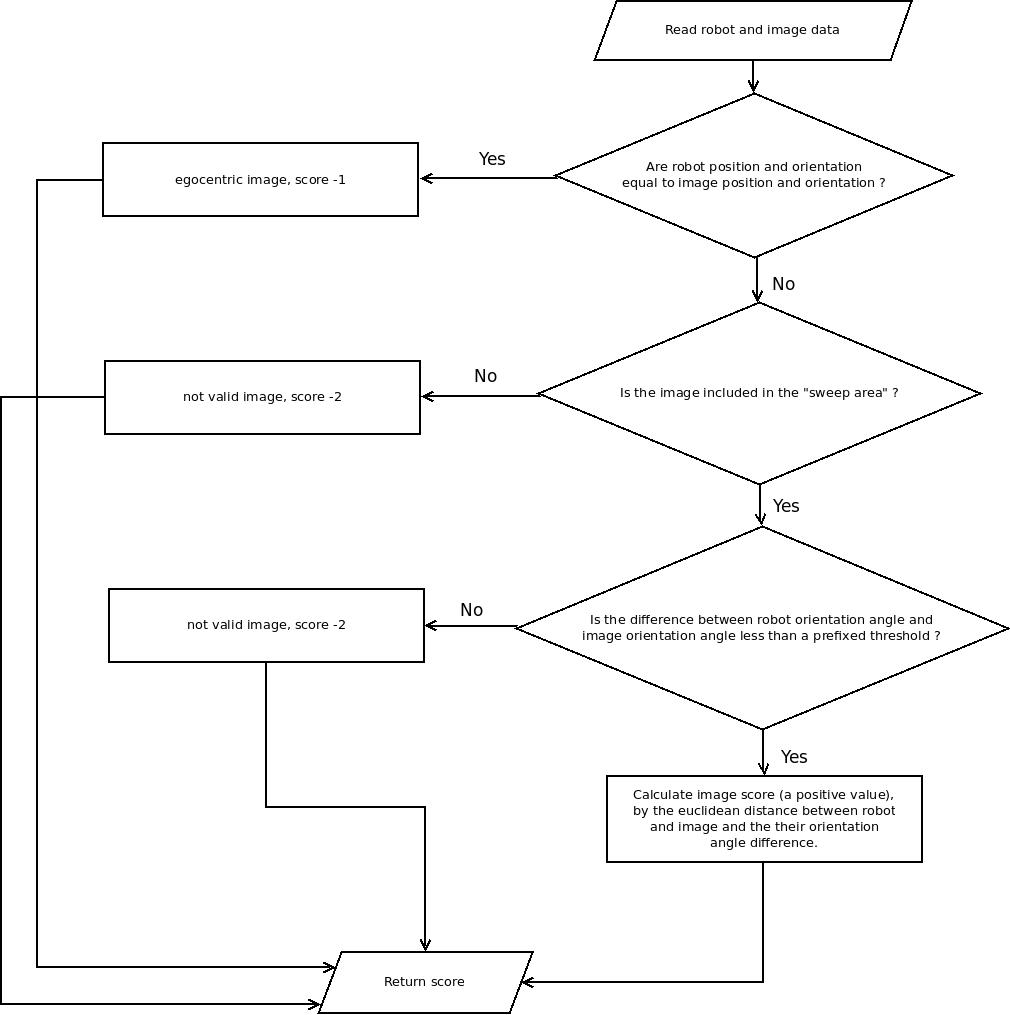
\includegraphics[width=400pt]{img/sweep_angle_diagram.jpeg} 
    \caption{Sweep angle diagram}
    \label{fig:sweep_angle_diagram}
  \end{center}
\end{figure}

%
The function to evaluate the score from the difference between the two angles is a Gaussian function centre
in zero. The return value will be therefore always a positive number.
%

%
The use of a Gaussian function allows to obtain different values even for two very close angle difference
(Gaussian is a injective function), regardless of the assigned variance. Moreover, it is defined for all real
numbers.
In this way is always possible to discern the best angle difference, by choosing the highest value returned by
the function.
%

%
Finally, we have to take in account the euclidean distance between the image and the robot. If the distance is
zero, we are examining the egocentric image. On one side, the images too close to the robot will be coupled
with a low score, because they are too similar to the egocentric one. On the other side, the images too far
from the robot will be coupled again with a low score, because they would show the robot too distance to
teleguide it properly.
%

%
The preferable image would distance from the robot a predefined quantity, specified by the user. This value
indicate us where to centre another Gaussian function, in order to obtain the score from the distance between
image and robot. The more the image is close to the preferred distance, the more the score assigned will be high.
%

%
The reasons that justifies the use of the Gaussian function are the same previously explained for the angle
difference. The values obtained from the two Gaussian functions, after adding them, form the global score.
%

%
To summarize the method above described (illustrated in figure \ref{fig:sweep_angle_diagram}), we coupled
every image with a score: the one with the maximum value will be chosen and put as background. If the image is
not included in the sweep area (defined by a sweep angle and therefore by the "c" and "d" line) it has to be
discarded. The score assigned will be -2.
%

%
The images situated within the sweep area, but with an orientation angle that differs too much from the robot
orientation angle, have to be discarded as the previous one: the score assigned will be -2 again.
If the image position and orientation coincide with robot position and orientation, the image represents the
egocentric vision. We remember that in our set there will always be the egocentric image, and that this will be
choose as background when no other image for exocentric vision are available. The score coupled with the egocentric 
vision will be -1.
%

%
Finally, all the other images - if present - are coupled with a positive number, because obtained by the sum of
values calculated with Gaussian functions. The most high score indicate the better image to chose as background;
if there are no preferable images, the image with -1 (i.e. the egocentric image) will be chosen.
%

%
Because the DataLogic is designed to choose the image with the minimum score and not with maximum, all we have to
do is multiply every score for -1 before returning it: in this way we convert a maximum research in a minimum one.
%

%
\paragraph{The WithinBoundaries algorithm}
